\documentclass[sigconf]{acmart}
% Local preview support; replace with the organizer's preamble when available.
\newif\ifguideStyle
\newcommand{\guide}[1]{%
  \ifguideStyle
    {\color{gray!65}\itshape #1}%
  \fi
}

\guideStylefalse
\setcopyright{none}
\settopmatter{printacmref=false}
\acmConference[Technical Report]{Competition Technical Report}{November 2026}{Online}
\acmYear{2026}
\acmDOI{}
\acmISBN{}
\setlength{\emergencystretch}{1em}
\setcounter{dbltopnumber}{3}
\renewcommand{\dbltopfraction}{0.99}
\renewcommand{\textfraction}{0.01}
\setlength{\dblfloatsep}{3pt}
\setlength{\dbltextfloatsep}{4pt}
\setlength{\textfloatsep}{5pt}

\begin{document}
\title{Solar Filament Instance Segmentation in H-Alpha Images}
\subtitle{Technical Report for the Solar Filament Segmentation Challenge 2026}
\author{Gregory Kojadinovich II}
\affiliation{%
  \institution{Europa Waters LLC}
  \city{South Lake Tahoe, CA}
  \country{USA}
}
\email{gregkoja3343@icloud.com}

\begin{abstract}
I evaluate four segmentation pipelines on the Solar Filament Segmentation
Challenge. Public panoptic quality (PQ) increases from 0.29 for a ResNet18
U-Net baseline to 0.32 after higher-resolution fine-tuning, 0.35 for a
YOLO11s-segementation detector with crop refinement and mask repair, and 0.36
for a five-fold YOLO/ResNet34-U-Net ensemble. The experiments change multiple
factors; the progression is not a controlled ablation. I describe the data
split, model configurations, ensemble, and limits of the available evidence.
\end{abstract}

\begin{teaserfigure}
\centering
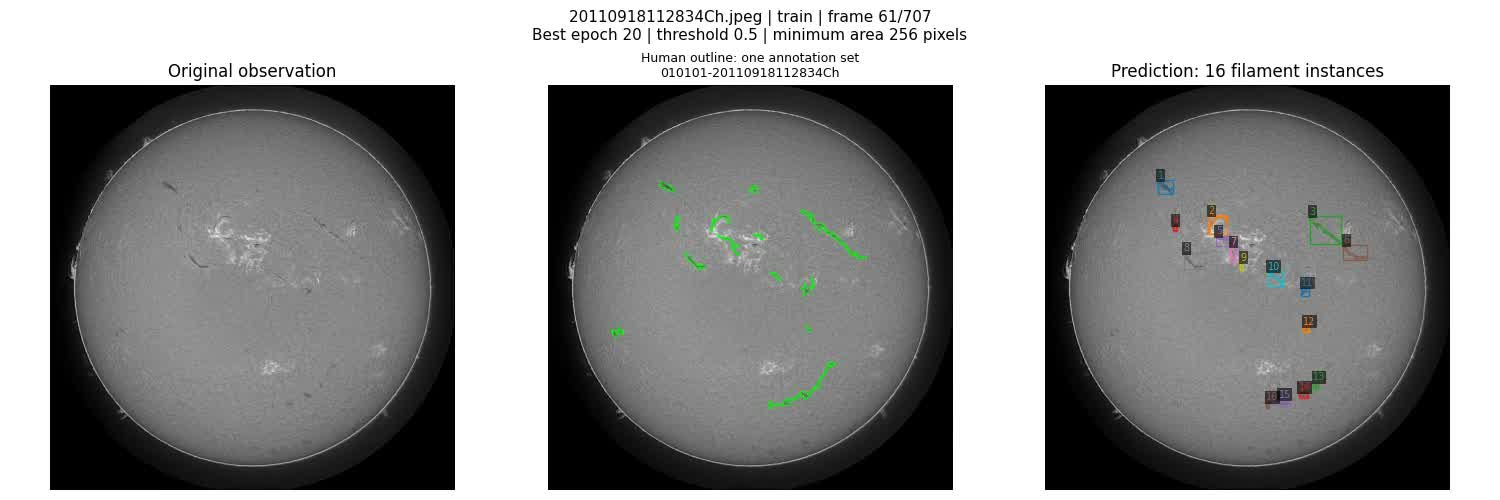
\includegraphics[width=0.85\textwidth]{../Baseline Video/thumbnail.jpg}
\caption{Baseline V1 review frame with observation, annotation, and model
overlay.}
\label{fig:baseline}
\end{teaserfigure}
\maketitle

\begin{figure*}[t]
\centering
\large
\begin{tabular}{cccc}
\shortstack{0.29\\\textcolor{blue!65!black}{\rule{1.1cm}{14.5mm}}\\V1} &
\shortstack{0.32\\\textcolor{orange!85!black}{\rule{1.1cm}{16mm}}\\V2} &
\shortstack{0.35\\\textcolor{green!50!black}{\rule{1.1cm}{17.5mm}}\\V3} &
\shortstack{0.36\\\textcolor{purple!70!black}{\rule{1.1cm}{18mm}}\\V5}
\end{tabular}

\smallskip
\normalsize
\begin{tabular}{lllll}
\hline
Run & Main model & Image size & Refiner & GPU \\
\hline
V1 & ResNet18 U-Net & 512 px & No & T4x2 \\
V2 & ResNet18 U-Net & 1024 px & No & T4x2 \\
V3 & YOLO11s-seg & 1024 px & ResNet18 U-Net & T4x2 \\
V5 & 5 $\times$ YOLO11s-seg & 1024 px & ResNet34 U-Net, fold-selected & T4x2 \\
\hline
\end{tabular}
\caption{Public PQ and pipeline summary. Runtimes for V1 and V2 are their
recorded training-stage times; V2 fine-tunes V1. V3 also completed four
refiner epochs; its detector ran for 1.254 hours. V5's completed run exceeded
two hours, but its total training time and completed epoch counts are
unavailable.}
\label{fig:scores}
\end{figure*}

\section{Context}
The challenge uses grayscale GONG H-$\alpha$ intensity images and
annotator-specific filament masks~\cite{filament-segmentation-2026,ahmadzadeh2024dataset}.
The objective is to produce separate, nonoverlapping filament instances.


The related ESAIR poster addresses filament boundaries, grouping, and
chirality classification~\cite{esairposter2026}; those methods are not
implemented here. H-Alpha Anomalyzer studies observation-quality
anomalies~\cite{khazaei2025software,khazaei2025icdm}; a broader review
surveys anomaly detection~\cite{ruff2021anomaly}. These are contextual
references, not filament segmentation results for this pipeline.

Two public U-Net notebooks were reviewed for comparison~\cite{pavlonotebook,foysalnotebook}.
The V3 detector/refiner design was informed by a public YOLO/U-Net
notebook~\cite{ektarrnotebook}; our implementation uses a different U-Net,
day-grouped splits, and separate annotator targets. No score parity is claimed.

\begin{figure*}[t]
\centering
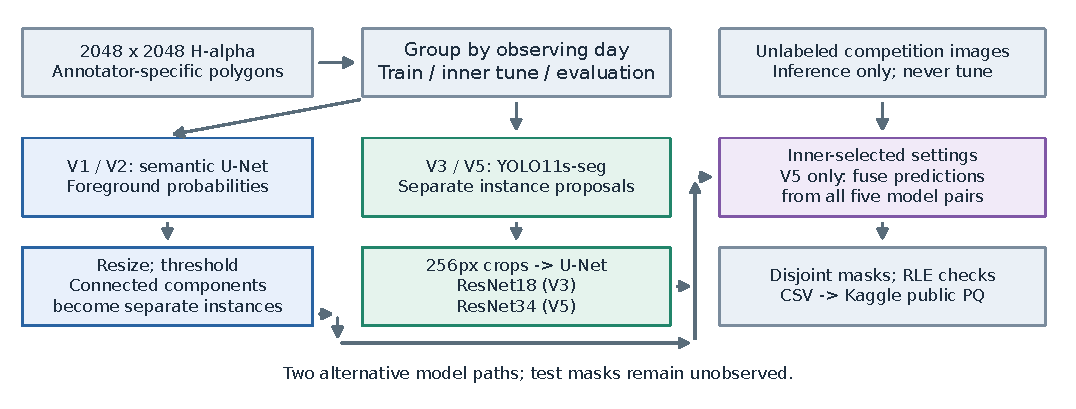
\includegraphics[width=0.80\textwidth]{figures-v2/workflow.pdf}
\caption{U-Net Semantic Segmentation Computer Vision ML pipelines. Training, tuning, and test
inference are distinct image sets fed to the pipeline.}
\label{fig:workflow}
\end{figure*}

\begin{figure*}[t]
\centering
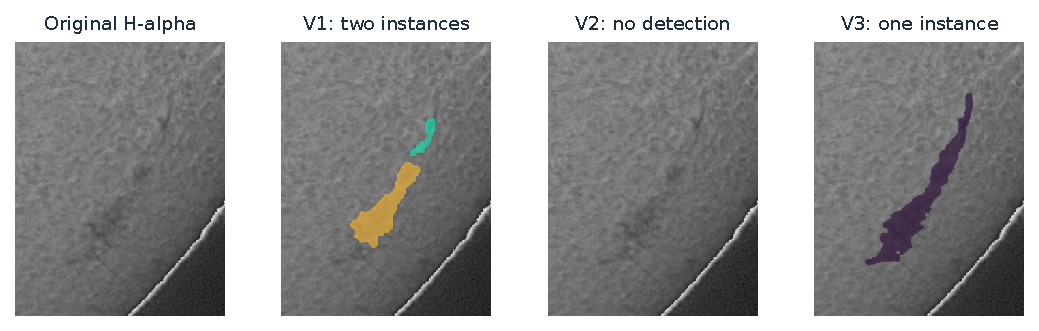
\includegraphics[width=0.80\textwidth]{figures-v2/mask_comparison.pdf}
\caption{Predictions for a disagreement-selected test crop
(\texttt{20210708060030Lh.jpeg}, $x=[1502,1767)$, $y=[1328,1673)$).
Colors identify predicted instances, not ground truth or correctness.}
\label{fig:masks}
\end{figure*}

\begin{figure*}[t]
\centering
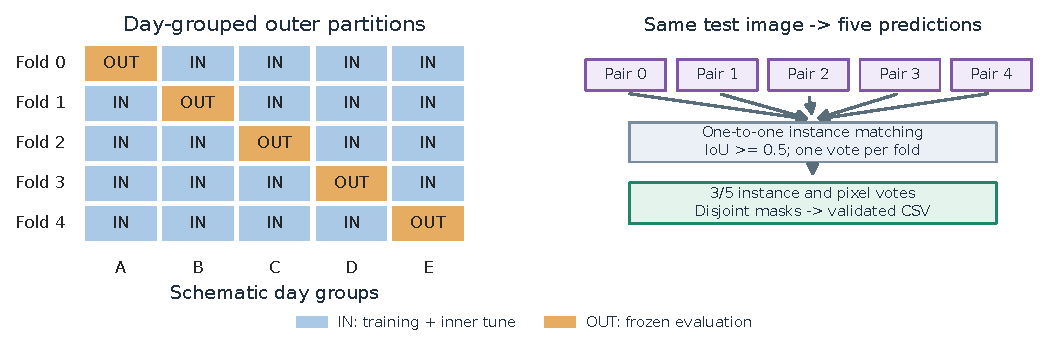
\includegraphics[width=0.80\textwidth]{figures-v2/folds_and_fusion.pdf}
\caption{Schematic day-grouped folds and five-model matching and voting.
Each IN partition includes training and inner tuning; OUT is held out.}
\label{fig:folds}
\end{figure*}

\begin{figure*}[t]
\centering
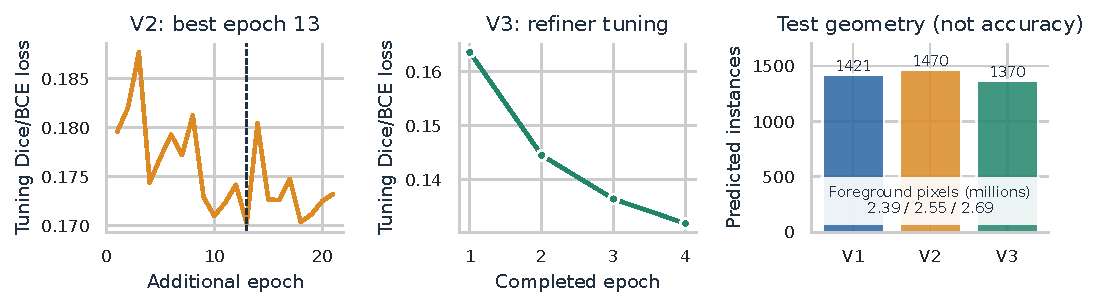
\includegraphics[width=0.80\textwidth]{figures-v2/training_and_geometry.pdf}
\caption{V1, V2, and V3 prediction diagnostics..}
\label{fig:diagnostics}
\end{figure*}

\section{Data and Evaluation}
The competition data comprise 707 labeled photographs, 1,154 annotator image
sets, 8,199 instances, and 180 unlabeled test images. V1--V3 use a fixed
day-grouped split of 499 training, 103 tuning, and 105 holdout photographs
(seed 2026). All annotation sets for a photograph remain together. Local
metrics average annotators within photographs, then photographs.

Panoptic quality combines instance recognition and overlap~\cite{pq}:
\begin{equation}
 \mathrm{PQ}=
 \frac{\sum_{(p,g)\in TP}\mathrm{IoU}(p,g)}
 {|TP|+\tfrac12|FP|+\tfrac12|FN|}.
\end{equation}
Local matching requires IoU strictly greater than 0.5. The public PQ scores
are single-run measurements; no repeated-seed uncertainty is available.

\section{Models and Results}
\subsection{V1: Semantic Baseline}
A U-Net~\cite{unet} with an ImageNet-pretrained ResNet18 encoder~\cite{resnet}
predicts foreground probabilities at 512 pixels per side. Training uses
AdamW, batch 8, 20 epochs, and equal-weight Dice/BCE loss. Thresholding and
eight-connected components produce instances. Submission 58301531 scores
0.29 PQ. Connected components can merge touching filaments or split
disconnected structures.

\subsection{V2: Higher-Resolution Fine-Tuning}
Focused V2 fine-tunes V1 at 1024 pixels with CLAHE~\cite{opencvclahevisual},
batch 2, and AdamW learning rate $10^{-4}$. It selects additional epoch 13
and stops at 21. Submission 58304132 scores 0.32 PQ. Resolution, contrast,
and training schedule changed together.

\subsection{V3: Instance Proposals and Refinement}
YOLO11s-seg~\cite{ultralyticsvisual} proposes instances at 1024 pixels; a
ResNet18 U-Net refines $256\times256$ crops. The refiner cannot recover
instances missed by the detector. The detector completed 47 epochs and part
of epoch 48; the refiner completed four epochs. The original CSV was rejected
for overlapping masks. Offline repair removed contested pixels without
retraining; submission 58316663 scores 0.35 PQ.

\subsection{V5: Five-Fold Ensemble}
V5 trains five independent YOLO11s-seg/ResNet34-U-Net pairs on day-grouped
folds. Each fold trains a ResNet34 refiner and uses an inner tuning split to
choose between YOLO-only and refined output, as well as confidence and area
thresholds. The outer holdout is not used for
selection~\cite{varma2006}. Per-fold ceilings are five detector and two
refiner epochs. Fold 4's refiner required recovery without a deadline;
the completed run exceeded its two-hour target.

For each test image, the five models predict using their selected settings.
One-to-one instance matching uses IoU at least 0.5; instances and pixels
require three of five votes. Small remnants are filtered and overlaps
removed. The ensemble has no separately trained parameters. Submission
58327117 scores 0.36 PQ. This score does not isolate the refiner's effect or
establish that it improved performance; the per-fold selections and training
cost require the saved run records.

\section{Discussion and Reproducibility}
\begin{figure*}[t]
\centering
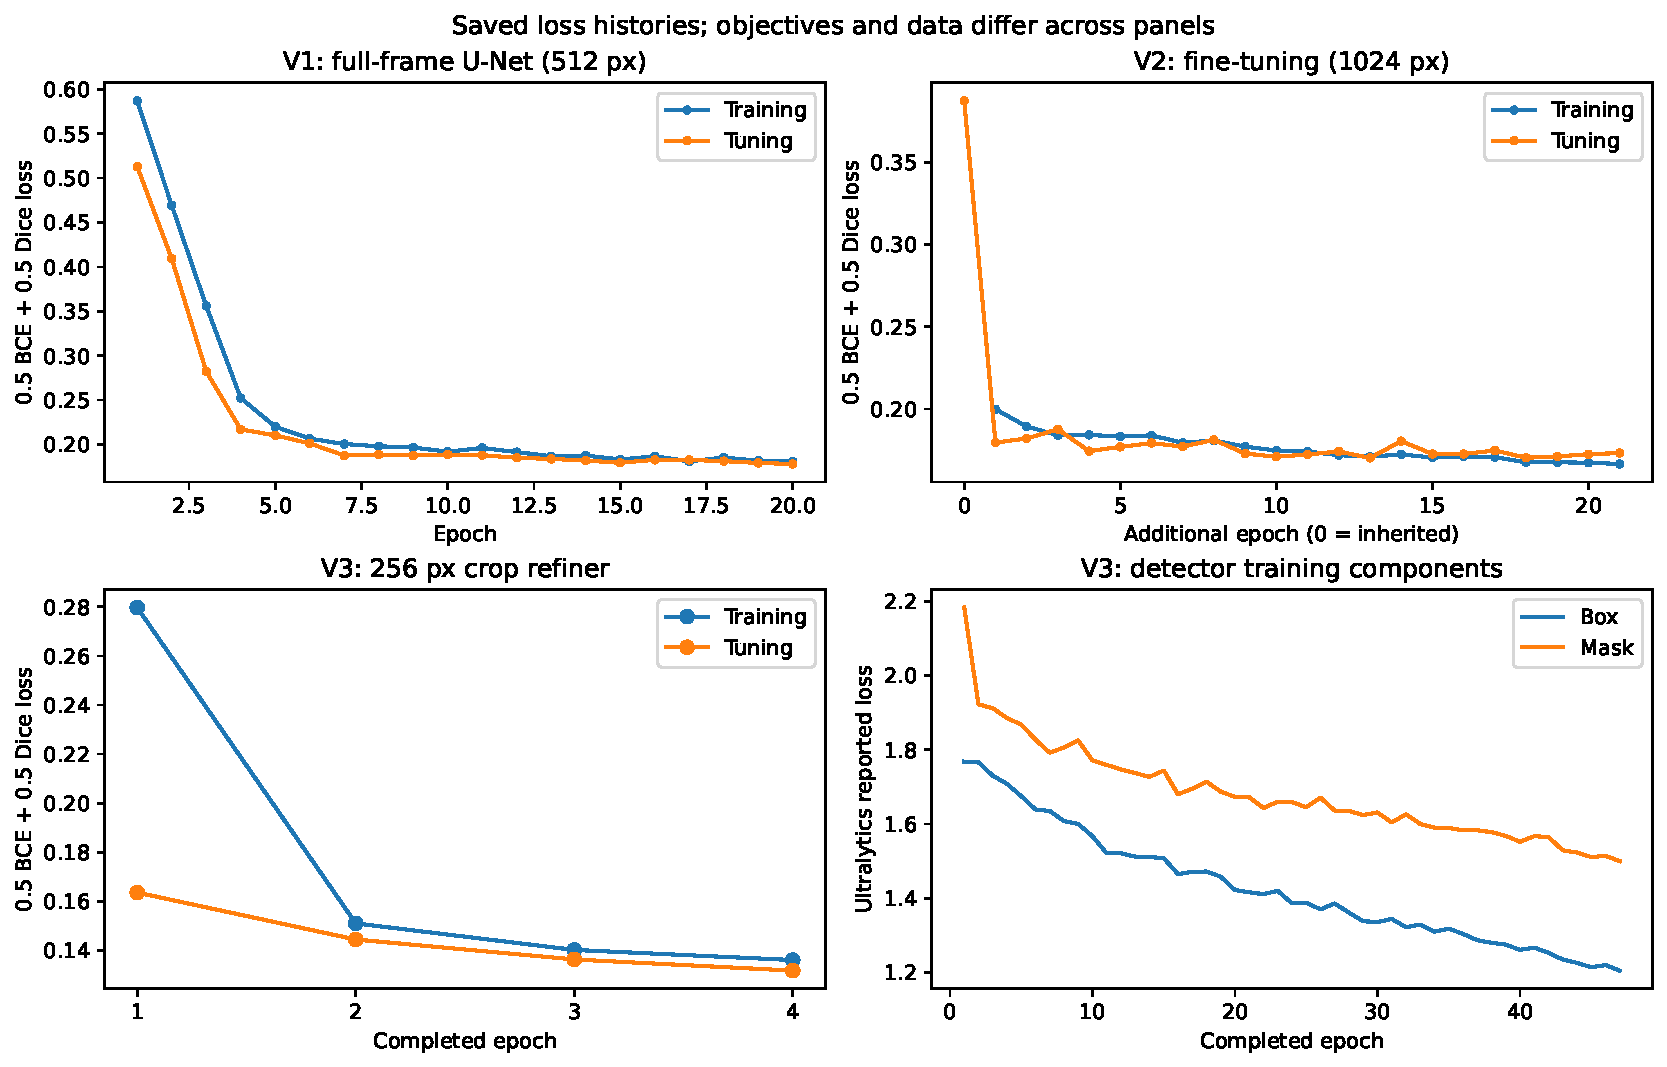
\includegraphics[width=\textwidth]{results-review/loss_by_epoch.pdf}
\caption{Saved training and tuning losses by epoch. V2 epochs are additional
to V1; V3 detector curves show distinct training loss components. Scored V5
histories are unavailable.}
\label{fig:loss}
\end{figure*}

The 0.07 absolute PQ increase from V1 to V5 reflects CV pipeline architecture changes. 

The training loss curves show the expected overall decline during
optimization. V1's best checkpoint was epoch 20, selected by its lowest
tuning loss. V2's training loss followed a relatively smooth downward
trend with small fluctuations, while its best tuning loss occurred at
additional epoch 13. Falling training loss alone does not establish
improved generalization.

Figure~\ref{fig:loss} shows V1 tuning loss reaches its minimum at epoch 20:
longer training merits testing. V2 reaches its minimum at additional epoch
13, then fluctuates; more epochs do not guarantee improvement. V3 refiner
tuning loss falls from 0.1636 to 0.1318 over four epochs before its budget
stop, motivating longer training without proving convergence. Detector loss
declines, but late validation metrics fluctuate. Full-image, crop and detector
losses are not directly comparable or substitutes for PQ. 

The accepted V5 CSV contains 1,127 masks across 177 images; three
images have no retained predictions. The
repository\footnote{\href{https://github.com/Greg-Kojadinovich/solar-filament-segmentation-2026}{Public source repository.}}
includes notebooks, the CSV, figures, and tests. Full reproduction still
requires the five checkpoint pairs, calibration and split plans, actual
environment, completed epoch counts, and run logs.

\section{Conclusions}
The YOLO-based pipelines scored 0.35 and 0.36 public PQ versus 0.29 and
0.32 for semantic baselines. I recommend YOLO for further study; these are
not controlled comparisons. Feature and threshold tuning with labeled error
analysis should investigate missed proposals, boundaries, fragmentation, and
overlap ownership. Longer refiner training may help but does not guarantee
improved PQ.

\section{Acknowledgment}
The Filament Segmentation Challenge 2026 is partially supported by the U.S.
National Science Foundation under grants 2209912, 2433781, and 2511630.
The challenge is sponsored by the U.S. National Science Foundation and
National Solar Observatory.

This work uses GONG data from the National Solar Observatory Integrated
Synoptic Program, operated by AURA under a cooperative agreement with the
National Science Foundation, with contributions from NOAA. The GONG network
is hosted by the Big Bear Solar Observatory, High Altitude Observatory,
Learmonth Solar Observatory, Udaipur Solar Observatory, Instituto de
Astrofisica de Canarias, and Cerro Tololo Inter-American Observatory.

\bibliographystyle{ACM-Reference-Format}
\bibliography{main,poster_v2,references_v3}
\end{document}
